% DEFINED:   sec:heteroscedastic, fig:ch02-heteroscedastic
% RESOLVED:  (none new beyond ch02 internals)
% FORWARD:   (none)

\section{Uncertainty: heteroscedastic Gaussian NLL}\label{sec:heteroscedastic}

\Cref{ch:foundations}'s MSE loss assumed Gaussian errors with
\emph{constant} variance, absorbed into the loss constant. That is fine
when the noise really is constant. When the noise is input-dependent the
model has no way to report it. A point prediction does not say ``I am
confident here'' or ``I am unsure here.'' The user has to find that out
the hard way.

Heteroscedastic Gaussian regression fixes this with a two-output head.
The network outputs $(z_\mu, z_s)$ per example, and the loss interprets
them as the parameters of a per-input Gaussian:
\[
  \mu = z_\mu, \qquad \sigma = \mathrm{softplus}(z_s).
\]
Softplus, $\mathrm{softplus}(z) = \log(1 + e^z)$, is the smooth
analogue of the positive part. It guarantees $\sigma > 0$ for any
$z_s \in \mathbb{R}$, without clamping; its derivative is the logistic
sigmoid, $\mathrm{softplus}'(z) = \sigma_{\mathrm{logistic}}(z)$.

\textbf{NLL} (dropping the $\tfrac{1}{2}\log(2\pi)$ constant):
\[
  L = \frac{(y - \mu)^2}{2\sigma^2} + \log \sigma.
\]
The first term is the familiar squared error, rescaled by the predicted
precision $1/\sigma^2$. A confident prediction (small $\sigma$) gets a
\emph{larger} MSE-like gradient. The second term prevents the model from
inflating $\sigma$ to infinity to wash out the first term.

\textbf{Gradients,} hand-derived:
\[
  \frac{\partial L}{\partial \mu} = \frac{\mu - y}{\sigma^2}.
\]
The MSE gradient, scaled by predicted precision.
\[
  \frac{\partial L}{\partial \sigma} = -\frac{(y - \mu)^2}{\sigma^3} + \frac{1}{\sigma}.
\]
Zero when $(y - \mu)^2 = \sigma^2$: the maximum-likelihood point, where
the model sets $\sigma$ equal to the realized residual.

Chaining through softplus to get the gradient with respect to the
network output $z_s$:
\[
  \frac{\partial L}{\partial z_s}
    = \frac{\partial L}{\partial \sigma} \cdot \sigma_{\mathrm{logistic}}(z_s).
\]

\textbf{In \texttt{scratchnn}:}

\begin{lstlisting}
def softplus(z):
    """Softplus: log(1 + exp(z)). The smooth analogue of the positive part.

    Evaluated as max(z, 0) + log1p(exp(-|z|)) to avoid overflow for large |z|.
    Its derivative is the logistic sigmoid, sigmoid(z).
    """
    return max(z, 0.0) + math.log1p(math.exp(-abs(z)))


class GaussianNLLLoss(Loss):
    """Heteroscedastic Gaussian NLL. Expects two logits, (z_mu, z_s).

    The first logit is the mean mu = z_mu (identity link on the mean). The
    second logit z_s is mapped through softplus to a positive scale,
    sigma = softplus(z_s), enforcing positivity without clamping. Target y
    is a single real number. The constant 0.5 * log(2*pi) is omitted.

    Loss: 0.5 * (y - mu)**2 / sigma**2 + log(sigma).
    Gradients are hand-derived; the chain through softplus uses
    d(softplus(z_s))/dz_s = sigmoid(z_s).
    """

    def value(self, logits, y):
        mu = logits[0]
        s = softplus(logits[1])
        return 0.5 * (y - mu) ** 2 / (s * s) + math.log(s)

    def grad(self, logits, y):
        mu = logits[0]
        z_s = logits[1]
        s = softplus(z_s)
        dmu = (mu - y) / (s * s)
        ds = -((y - mu) ** 2) / (s ** 3) + 1.0 / s
        return [dmu, ds * sigmoid(z_s)]

    def probs(self, logits):
        # Report (mu, sigma) for the predictive Gaussian.
        return [logits[0], softplus(logits[1])]
\end{lstlisting}

The \texttt{softplus} helper is listed above in full; \texttt{GaussianNLLLoss}
has fifteen lines excluding docstring. Same \texttt{Loss} interface as the
other heads; the only novelty is that the head produces \emph{two} numbers
per example.

\textbf{Worked experiment.} A 1-D function with input-dependent noise:
$y = \sin(x) + \varepsilon$ where
$\varepsilon \sim \mathcal{N}(0, \sigma(x)^2)$ and
$\sigma(x) = |x|/3 + 0.1$ over $x \in [0, 6]$. Noise is small on the
left, growing to about $\sigma = 2$ on the right. Two networks of
identical body ($1 \to 16 \to 1$ for MSE, $1 \to 16 \to 2$ for
heteroscedastic), data seed~0, model seed~0, 300 epochs.
See \Cref{fig:ch02-heteroscedastic}.

\begin{figure}[h]
  \centering
  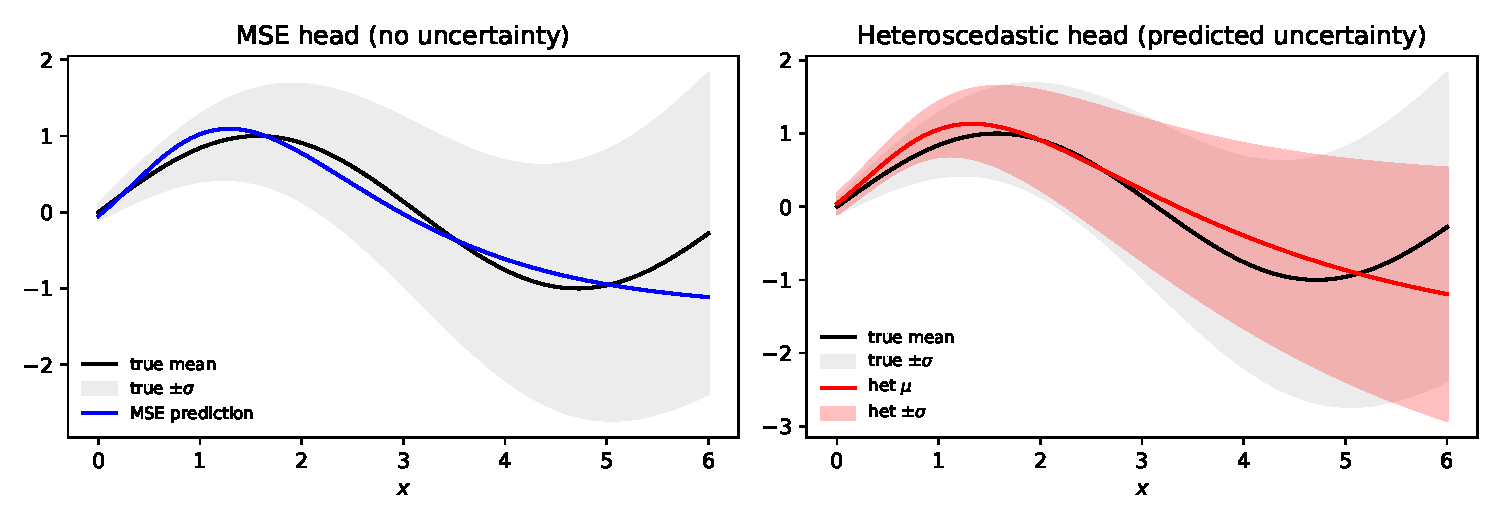
\includegraphics[width=0.92\linewidth]{figures/ch02-heteroscedastic.pdf}
  \caption{MSE head versus heteroscedastic Gaussian head.
    Left: MSE prediction (blue) against the true mean (black) with the
    true $\pm\sigma$ band (grey). The MSE model predicts only a mean.
    Right: heteroscedastic head, which predicts both a mean (red) and a
    per-input uncertainty band (pink). The predicted band tracks the
    true band closely, widening on the noisy right side.}
  \label{fig:ch02-heteroscedastic}
\end{figure}

\textbf{Findings:}

\begin{table}[h]
\centering
\begin{tabular}{r r r r r r}
\toprule
$x$ & true $\mu$ & true $\sigma$ & MSE pred & het $\mu$ & het $\sigma$ \\
\midrule
0.5 & 0.479 & 0.267 & 0.568 & 0.635 & 0.234 \\
1.5 & 0.997 & 0.600 & 1.059 & 1.114 & 0.525 \\
2.5 & 0.598 & 0.933 & 0.371 & 0.584 & 0.821 \\
3.5 & $-0.351$ & 1.267 & $-0.356$ & $-0.098$ & 1.115 \\
4.5 & $-0.978$ & 1.600 & $-0.806$ & $-0.650$ & 1.392 \\
5.5 & $-0.706$ & 1.933 & $-1.044$ & $-1.046$ & 1.625 \\
\bottomrule
\end{tabular}
\caption{Predictions at six query points. The heteroscedastic model
  recovers the input-dependent $\sigma$ within 10--15\% across the
  range. The MSE model has no $\sigma$ at all.}
\end{table}

The heteroscedastic model tracks the true $\sigma$ within 10--15\%
across the range. The MSE model has no $\sigma$ at all; it only predicts
the mean.

To compare on equal footing: fit a single global $\sigma$ for the MSE
model post-hoc (the RMS training residual), then compute Gaussian NLL on
the test set under each model's predicted distribution.

\begin{table}[h]
\centering
\begin{tabular}{lr}
\toprule
Model & Test Gaussian NLL \\
\midrule
MSE model + global $\sigma$ & 0.745 \\
Heteroscedastic head & 0.509 \\
\bottomrule
\end{tabular}
\caption{Test Gaussian NLL on 200 held-out samples (lower is better).
  Numbers regenerated from the paired notebook with seed~0.}
\end{table}

The heteroscedastic head improves test NLL by 0.24 nats per sample.
That is the calibration premium: predicting variance separately for
each $x$ is worth a quarter of a nat over the homoscedastic assumption
on this dataset. The qualitative gain is bigger than the numerical one.
The MSE model plus global $\sigma$ is overconfident on the noisy right
side and underconfident on the clean left side; the heteroscedastic head
is correct on both.

This is the cleanest demonstration in this chapter that the choice of
head buys something tangible (calibrated, input-dependent uncertainty)
that the standard head cannot provide.
